\section{Ternary}

This section introduces the \link{https://github.com/marcharper/python-ternary}{python-ternary package}. You'll need to install this with pip or conda to follow along. You can use this to make various plots in the two-dimensional simplex. That is, you can make triangle plots where a point in the triangle represents a particular multinomial distribution over three possible outcomes. That is, the triangle is a two-dimensional projection of the space $\left\{ \left(p_1,p_2,p_3 \right)\in \mathbb{R}^3: p_1+p_2+p_3 = 1 \text{ and } p_i \in [0,1] \text{ for }i=1,2,3 \right\}.$

\begin{center}
    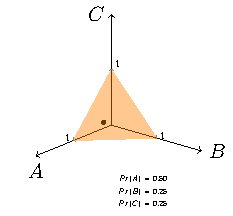
\includegraphics[width = .6\textwidth]{images/tikz_simplex_blank.pdf}
\end{center}

I encountered these diagrams in a few economics courses. Professor \link{https://www.ssc.wisc.edu/~whs/}{Bill Sandholm} made particularly memorable use of these diagrams in his courses and research in evolutionary game theory. These plots aren't the most natural selection for inclusion in this text. It's a personal indulgence and a favor to other game theorists.

After running \code{import ternary}, the construction of a plot isn't much different than what we covered in Chapter \ref{chapter:oop}. Start with figure and
\emph{ternary} axes objects. However, \code{ternary.figure()} will create both objects. There is no analogue to \code{plt.axes()} as this more closely imitates \code{plt.subplots(1,1)} than \code{plt.figure()}. It's not a perfect replica though. For example, there is no \code{figsize} parameter, but this can be adjusted with the figure method \code{set_size_inches}.

\pyfile{basic-ternary.py}

\begin{center}
    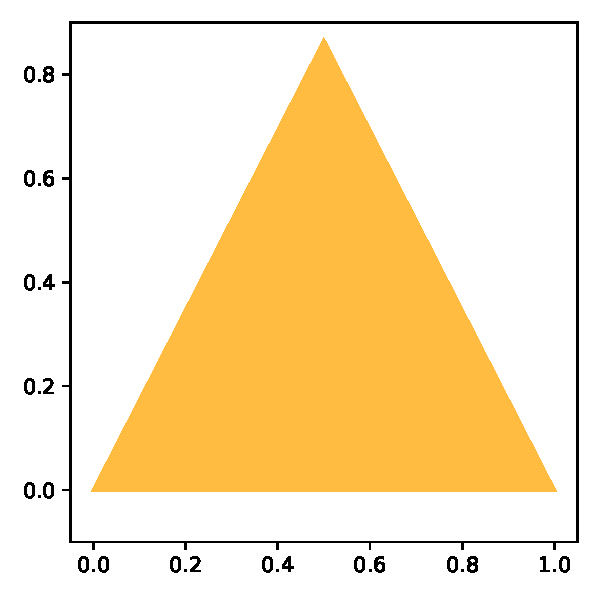
\includegraphics[width = .5\textwidth]{figures/specialplots/basic-ternary.pdf}
\end{center}

\pyfile{color-ternary.py}

\begin{center}
    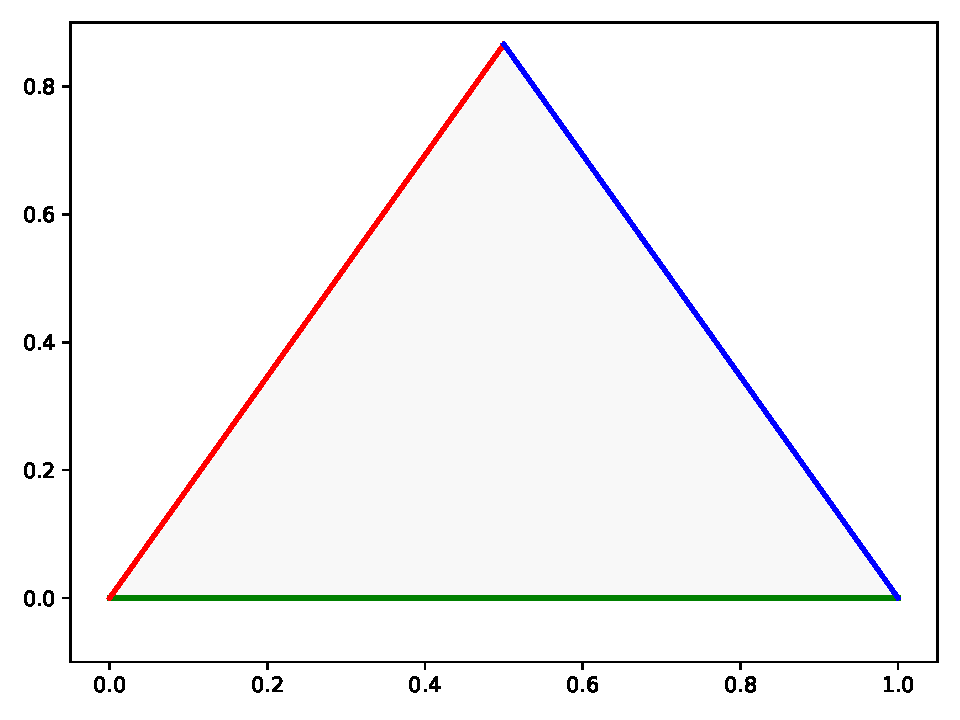
\includegraphics[width = .6\textwidth]{figures/specialplots/color-ternary.pdf}
\end{center}


Next, let's add some points with the \code{scatter} method, which works as you might expect. 

\pyfile{scatter-ternary.py}

\begin{center}
    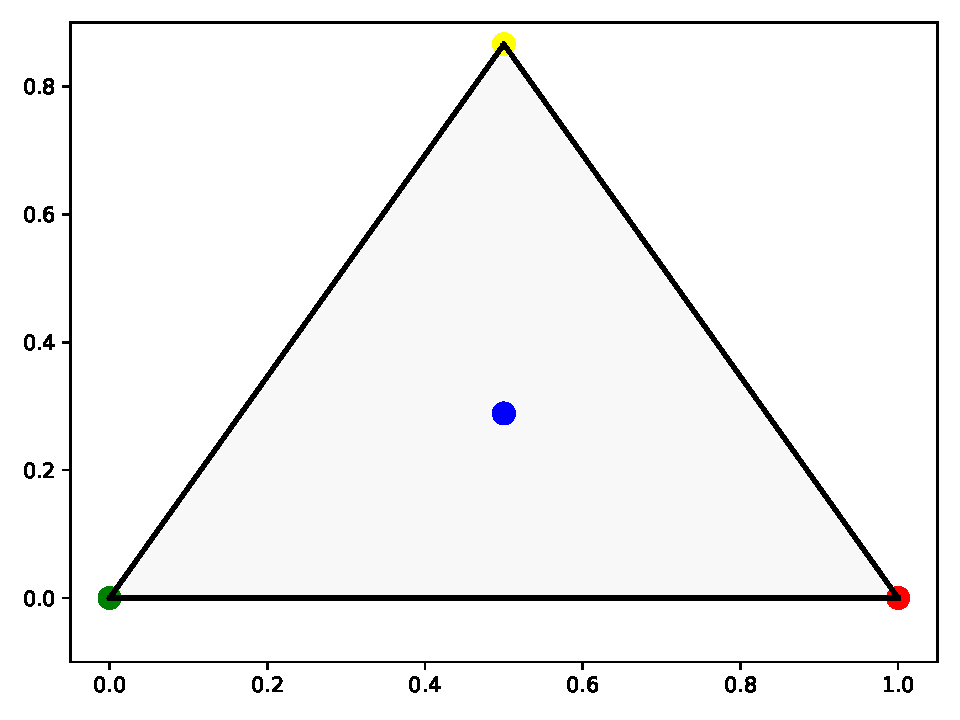
\includegraphics[width = .6\textwidth]{figures/specialplots/scatter-ternary.pdf}
\end{center}

The $x$- and $y$-axis ticks above correspond to the bottom and right axes, but this can be confusing since the $x,y$ point of $(0,0)$ is the point $(0,0,1)$ in the ternary plot. Accordingly, you might prettify the plot by removing those ticks and these axes entirely. This can be done with \code{tax.get_axes().axis('off')}. This works like \code{ax.axis} so we can also pass \code{'equal'} to equalize the axes. Adding gridlines with the \code{gridlines} method can also help the eye. This is demonstrated below. The horizontal gridlines correspond to the value along the right axis. The negatively sloped gridlines correspond to the left axis. The positively sloped gridlines correspond to the bottom axis. These gridlines are perpendicular to the direction of ascent along each axis and, just as for a typical plot, they show where the particular axis value is constant. 

\pyfile{grid-ternary.py}

\begin{center}
    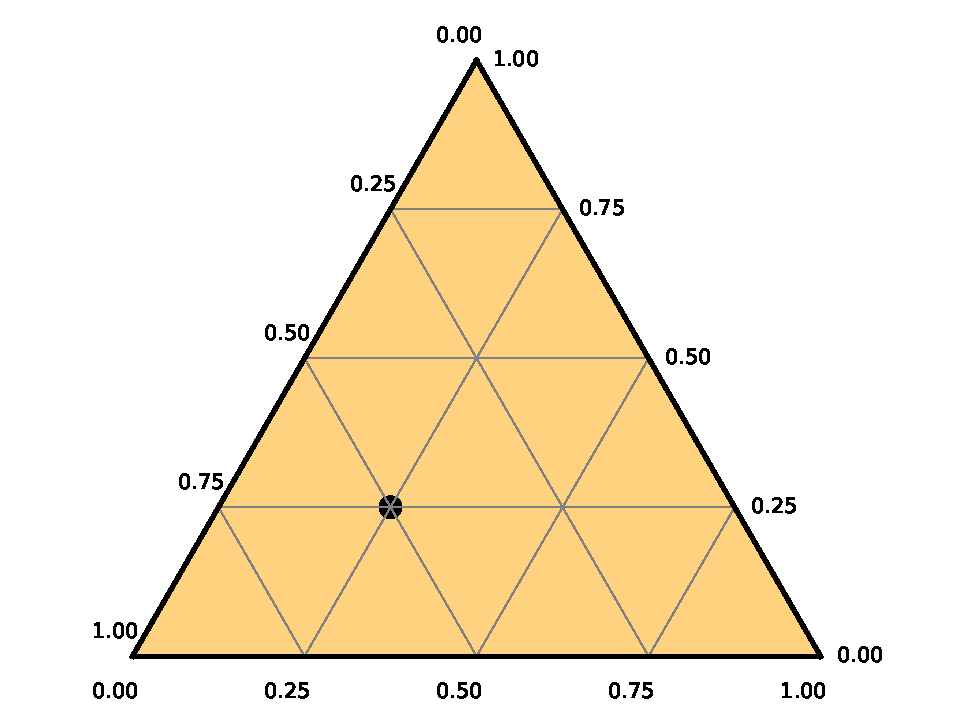
\includegraphics[width = .6\textwidth]{figures/specialplots/grid-ternary.pdf}
\end{center}


\section{Application: Rock, Paper, Scissors}

Throughout this chapter, we'll analyze the game rock paper scissors. If you need a reminder, there are two players who simultaneously choose an action of either rock, paper, or scissors. Rock beats scissors beats paper beats rock. Choosing the same action results in a tie. Your job is to choose an action based on your expectation of what your opponent will choose. 

First, we'll construct a heatmap to show the net winning percentage from choosing a particular action depending on the opponent's probability distribution over the three actions, so that a point in the simplex is that opponent's strategy and the color represents how often you win. The following is a function we'll use in making a heatmap, calculating the net winning percentage of an action against a particular distribution. 

\pyfile{rps-helper.py}

Now, we can create a heatmap using the function \code{winning_pct} and the \code{heatmapf} method. 

\pyfile{heat-rps.py}

\begin{center}
    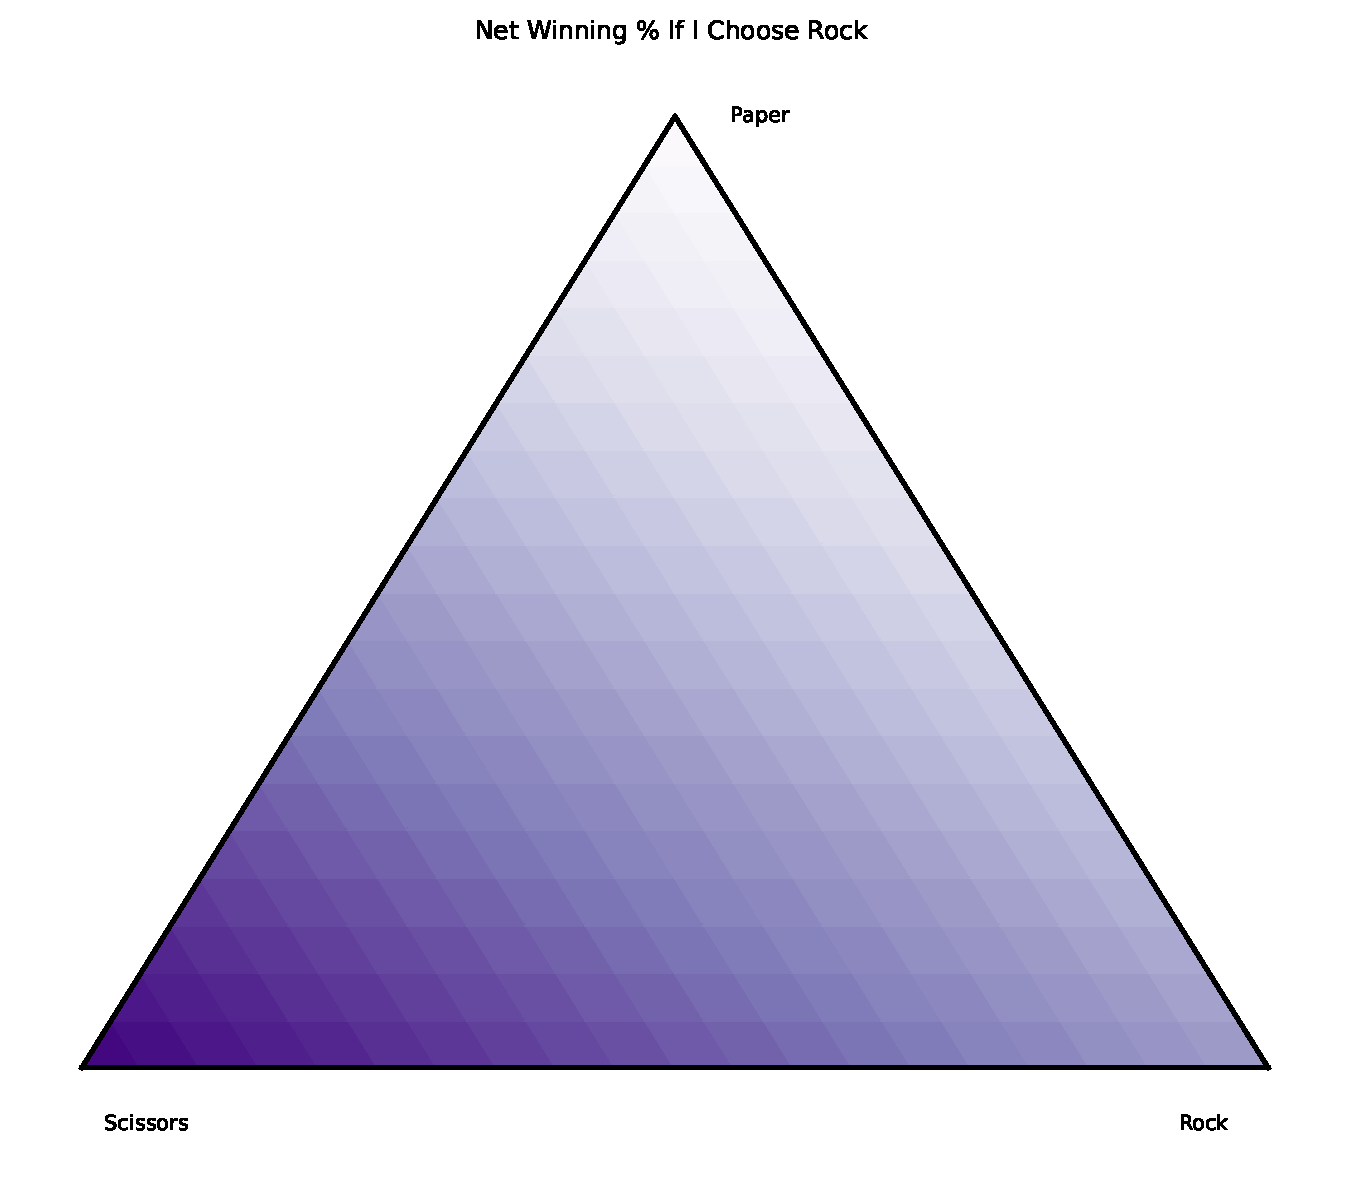
\includegraphics[width = 0.83\textwidth]{figures/specialplots/heat-rps.pdf}
\end{center}


The natural extension of the above might be to repeat the above, which supposes you choose rock, for the actions paper and scissors. This can be done straightforwardly, by changing the default action in the \code{winning_pct} function. For the game theorist, the more interesting question is, given my opponent's distribution over actions, what is my best response? The code below plots the regions of pairwise indifference between two actions. Then, we divide up the simplex into three best response regions. 

\pyfile{rps-br-lines.py}

\begin{center}
    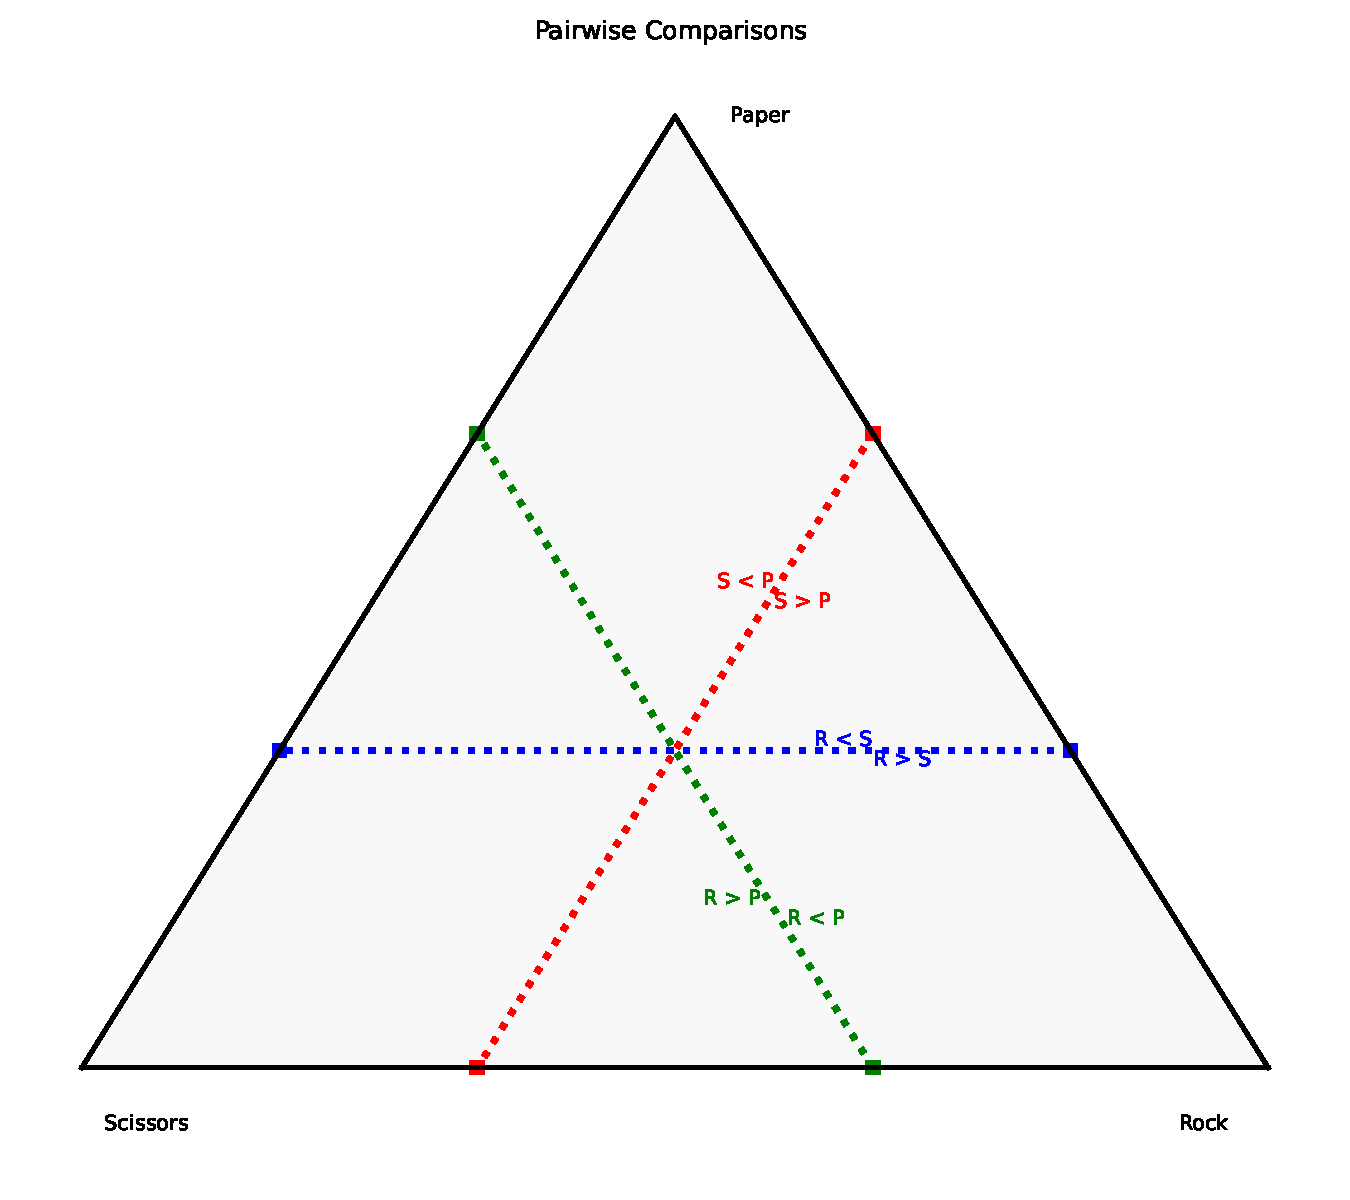
\includegraphics[width = 0.9\textwidth]{figures/specialplots/rps-br-lines.pdf}
\end{center}


We can color best responses zones by using the \code{heatmap} method, though it will take some work. First, we have some pure Python coding to do. Recall that \code{heatmap} requires a correspondence of points and the colors you want. We won't use a colormap, but we'll pass the colors in explicitly as RGBA values. This is a bit of a hack since the resulting plot and its colors won't have the ordered interpretation typical of heatmaps. 

\pyfile{rps-br-helper.py}

\pyfile{rps-br-zones.py}

\begin{center}
    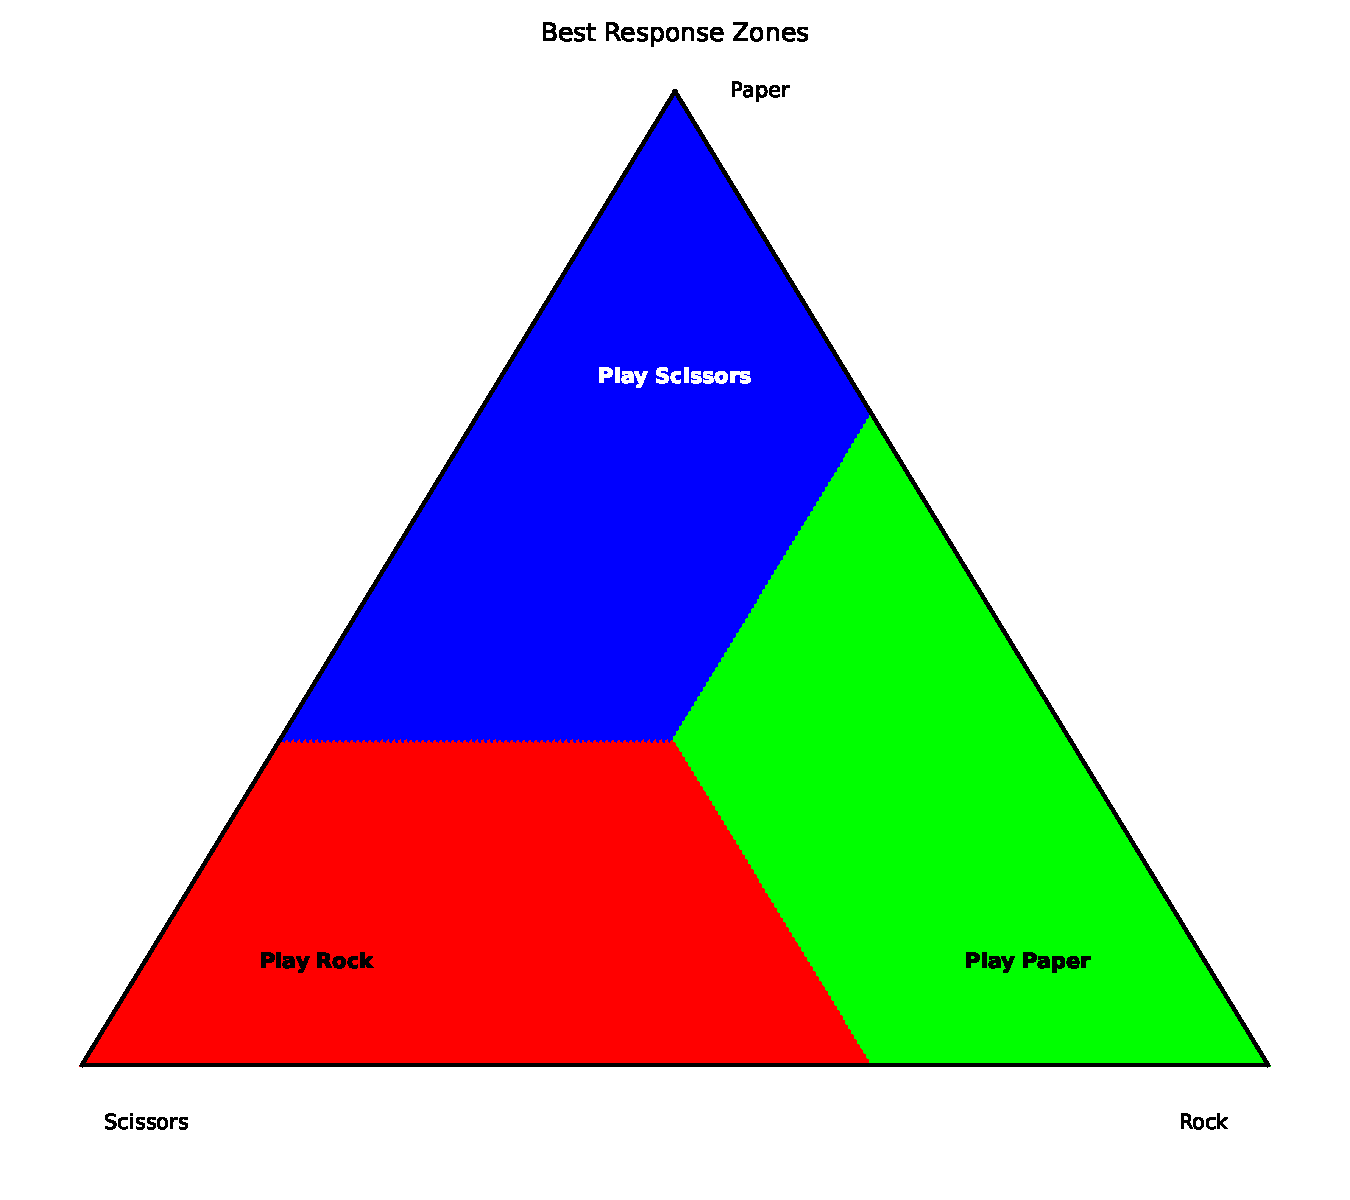
\includegraphics[width = 0.90\textwidth]{figures/specialplots/rps-br-zones.pdf}
\end{center}

Anyone inspecting what \code{data} looks like above will note that the points in the triangle aren't proper probability vectors as they add up to our \code{scale} value of 200 instead of one. That's immaterial for this application. A higher scale is chosen to create a sharper, exact border between between the best response regions. 